\documentclass{beamer}
\usepackage[utf8]{inputenc}

\usepackage{amsmath,amsfonts,amssymb,amsthm,
mathtools,mathrsfs}
\usepackage{physics}
\usepackage{xcolor}
\usepackage{hyperref}
\usepackage{caption}
\usepackage{subcaption}

\usepackage{tikz-cd} % arrow diagram

% Citation style
\usepackage[style=apa, backend=biber, natbib]{biblatex}
\addbibresource{references.bib}

\usetheme{Madrid}
\usecolortheme{default}
\useoutertheme[subsection=false]{miniframes}
\setbeamertemplate{frametitle continuation}{}
\setbeamertemplate{bibliography item}[triangle]
\setbeamertemplate{sidebar right}{}
\setbeamertemplate{caption}[numbered]
%\addtobeamertemplate{footnote}{}{\vspace{2ex}}

\addtobeamertemplate{block example begin}{%
    \setlength{\textwidth}{0.8\textwidth}
}{}

% Presenter notes
%\setbeameroption{show notes}



\title[DL for NFT Pricing]{Machine Learning for NFT Price Predictions}
%\subtitle{BUSN 41916 Bayes, AI, and Deep Learning}
\author{Mingxuan He}


\institute[]{
Booth School of Business, University of Chicago\\
mingxuanh@uchicago.edu
}


\date{\today}


\begin{document}


% title page
\begin{frame}
\titlepage  
\end{frame}


\section{Introduction}

\begin{frame}{Primer on NFTs}
    \begin{itemize}
        \item NFTs are unique digital assets (e.g. photos) stored on a blockchain.
        \item Mostly transacted using cryptocurrencies, predominantly Ethereum.
        \item Most NFTs are sold on ``marketplaces", grouped by ``collections"
    \end{itemize}
    \begin{figure}
        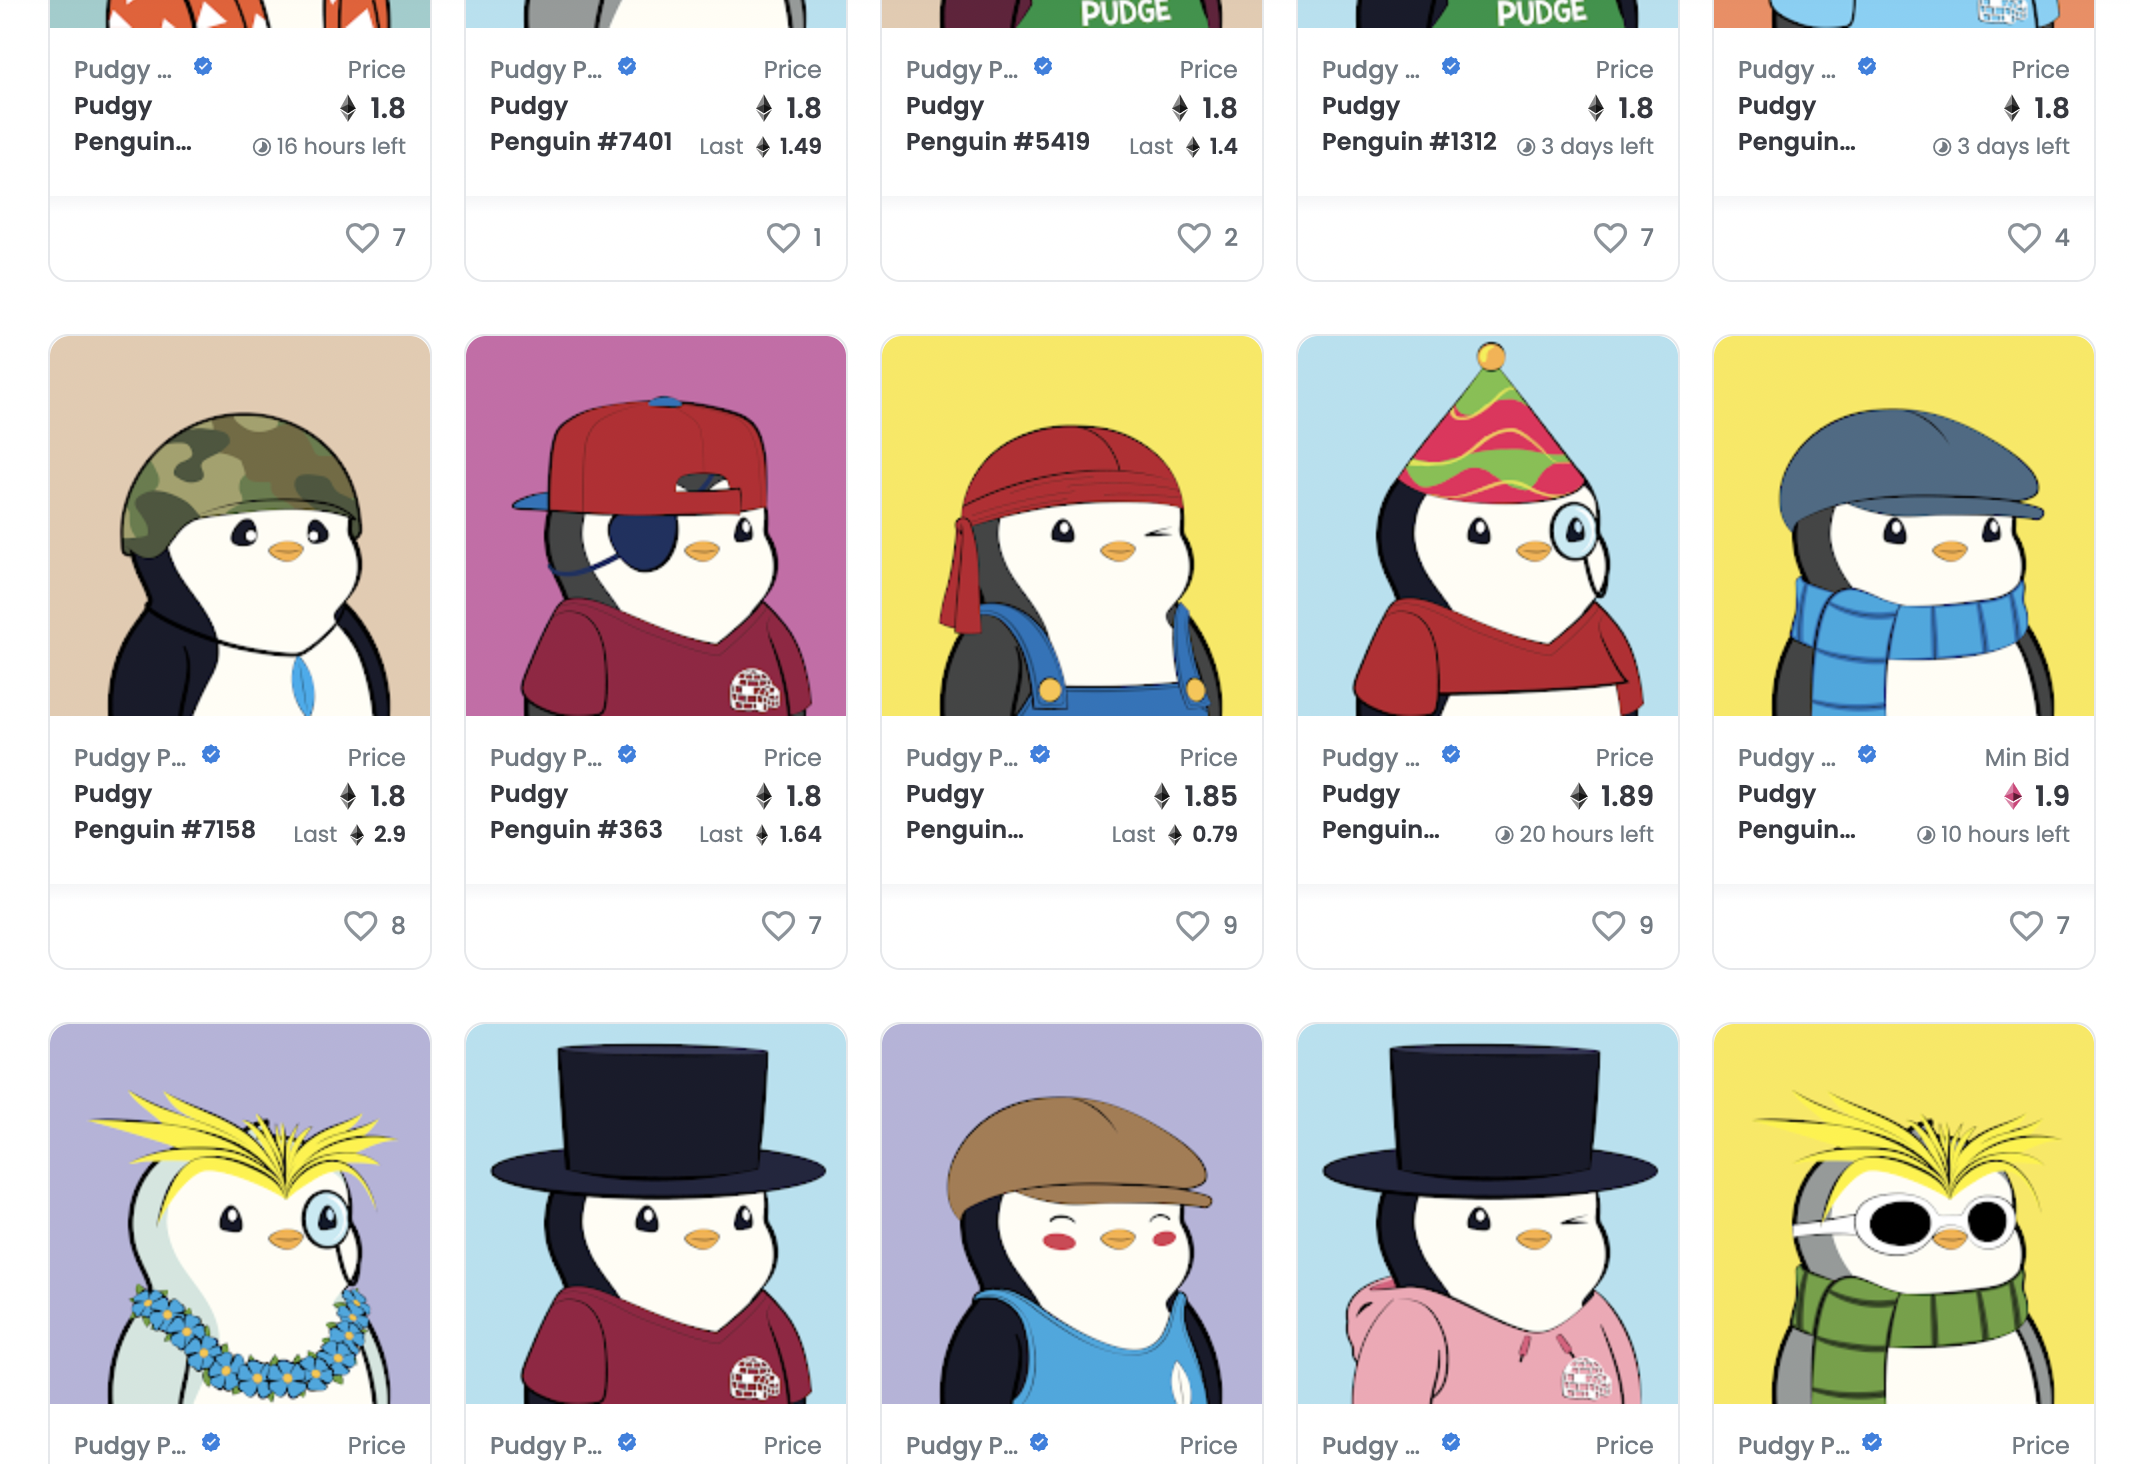
\includegraphics[width=0.6\textwidth]{../figures/penguins.png}
        %\captionsetup{labelformat=empty}
        \caption{\footnotesize{The Pudgy Penguins collection on OpenSea marketplace.}}
    \end{figure}
\end{frame}

\begin{frame}{Motivation}
    Various applications of NFT pricing models: Trading, decentralized borrowing/lending, tokenized real-world assets.\\
    \bigskip
    Literature:
    \begin{itemize}
        \item NFT prices co-moves with market trends \citep{nadini2021mapping,kong2021alternative,jain2022nft,kapoor2022tweetboost}
        \item High rarity drives up NFT prices \citep{mekacher2022heterogeneous,kong2021alternative}
    \end{itemize}

    Project goal:
    \begin{itemize}
        \item Build a ML model for a specific collection to predict the price of NFTs in real-time.
        \item Incorporate data on market prices and individual rarity.

    \end{itemize}
\end{frame}

\section{Data}
\begin{frame}{Data Sources}
    \begin{itemize}
        \item \textbf{Dune Analytics}\footnote{\url{https://dune.com}}: Public database of NFT trades on Ethereum.
        \item \textbf{OpenSea API}\footnote{\url{https://docs.opensea.io/reference/api-overview}}: Data from largest NFT marketplace on traits and rarity for each NFT in their collections.
    \end{itemize}

\end{frame}

\begin{frame}{Data Features}
    \begin{columns}[t]
        \column{0.4\textwidth}
        \begin{block}{Market features \\(by collection, daily)}
            \begin{itemize}
                \item Trading volume
                \item 5\% price
                \item Highest price
                \item Lowest price
            \end{itemize}
        \end{block}

        \begin{block}{Traits\\ (by NFT)}
            \begin{itemize}
                \item Background color
                \item Eyes
                \item ... (7 total)
            \end{itemize}
        \end{block}

        \column{0.4\textwidth}
        \begin{block}{Last sale\\ (by NFT)}
            \begin{itemize}
                \item Price of last sale
                \item Time since last sale
            \end{itemize}
        \end{block}
        \begin{block}{Rarity Rank\\ (by NFT)}
            \begin{itemize}
                \item Rarity rank within the collection\\
                (computed using OpenRarity Standard)
            \end{itemize}
        \end{block}

    \end{columns}
\end{frame}

\begin{frame}{Price history (Bored Apes)}
    \begin{figure}[t]
        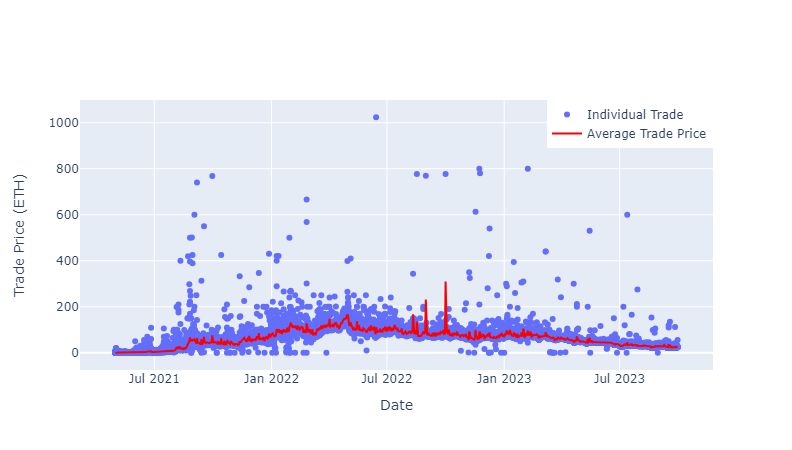
\includegraphics[width=0.8\textwidth]{../figures/price_date.png}
        \caption{Bored Apes: Historical trades.}
    \end{figure}
\end{frame}


\section{Modeling}

\begin{frame}{PCA analysis}
    \begin{figure}
        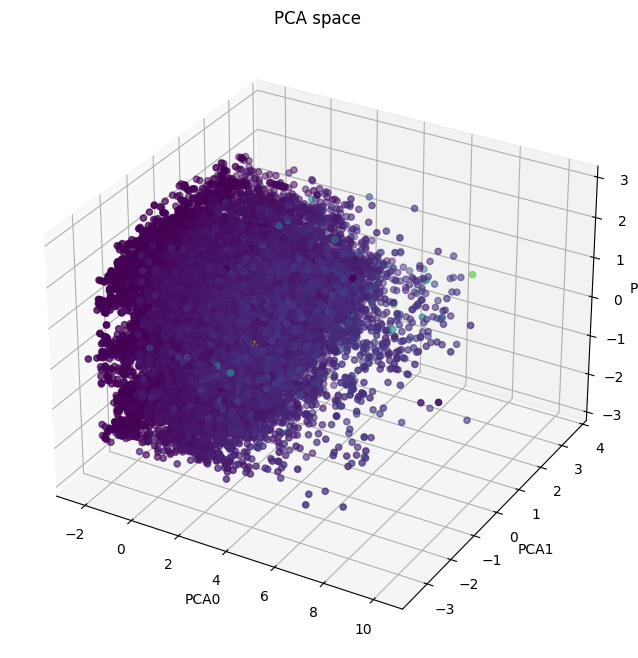
\includegraphics[width=0.5\textwidth]{../figures/pca_1.png}
        \caption{Bored Apes: Top 3 principal components.}
    \end{figure}
\end{frame}

\begin{frame}{Baseline Models}
    Framework: Python \texttt{sklearn} \\
    \begin{itemize}
        \item Linear models: OLS, Lasso, Ridge
        \item Tree-based models: Random Forest
    \end{itemize}
\end{frame}


\begin{frame}{Deep Learning Model}
    Framework: Python \texttt{tensorflow.keras} \\
    \begin{figure}
        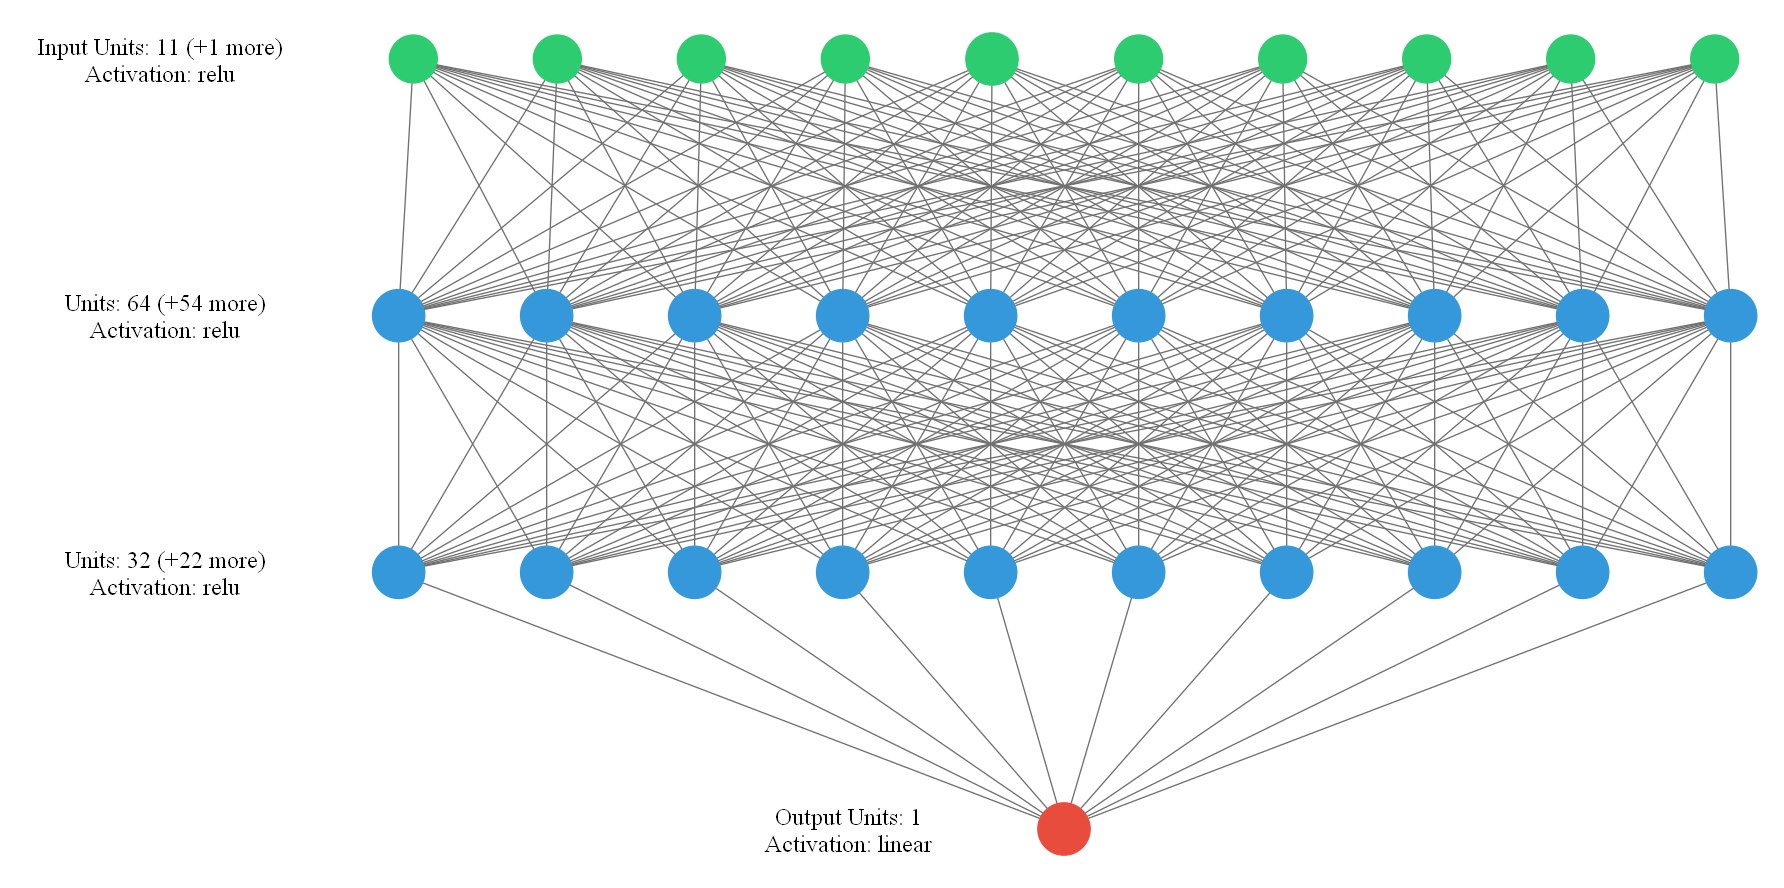
\includegraphics[width=\textwidth]{../figures/nn.png}
        \caption{Neural network architecture}
    \end{figure}
\end{frame}

\begin{frame}{NN Training}

\begin{figure}
    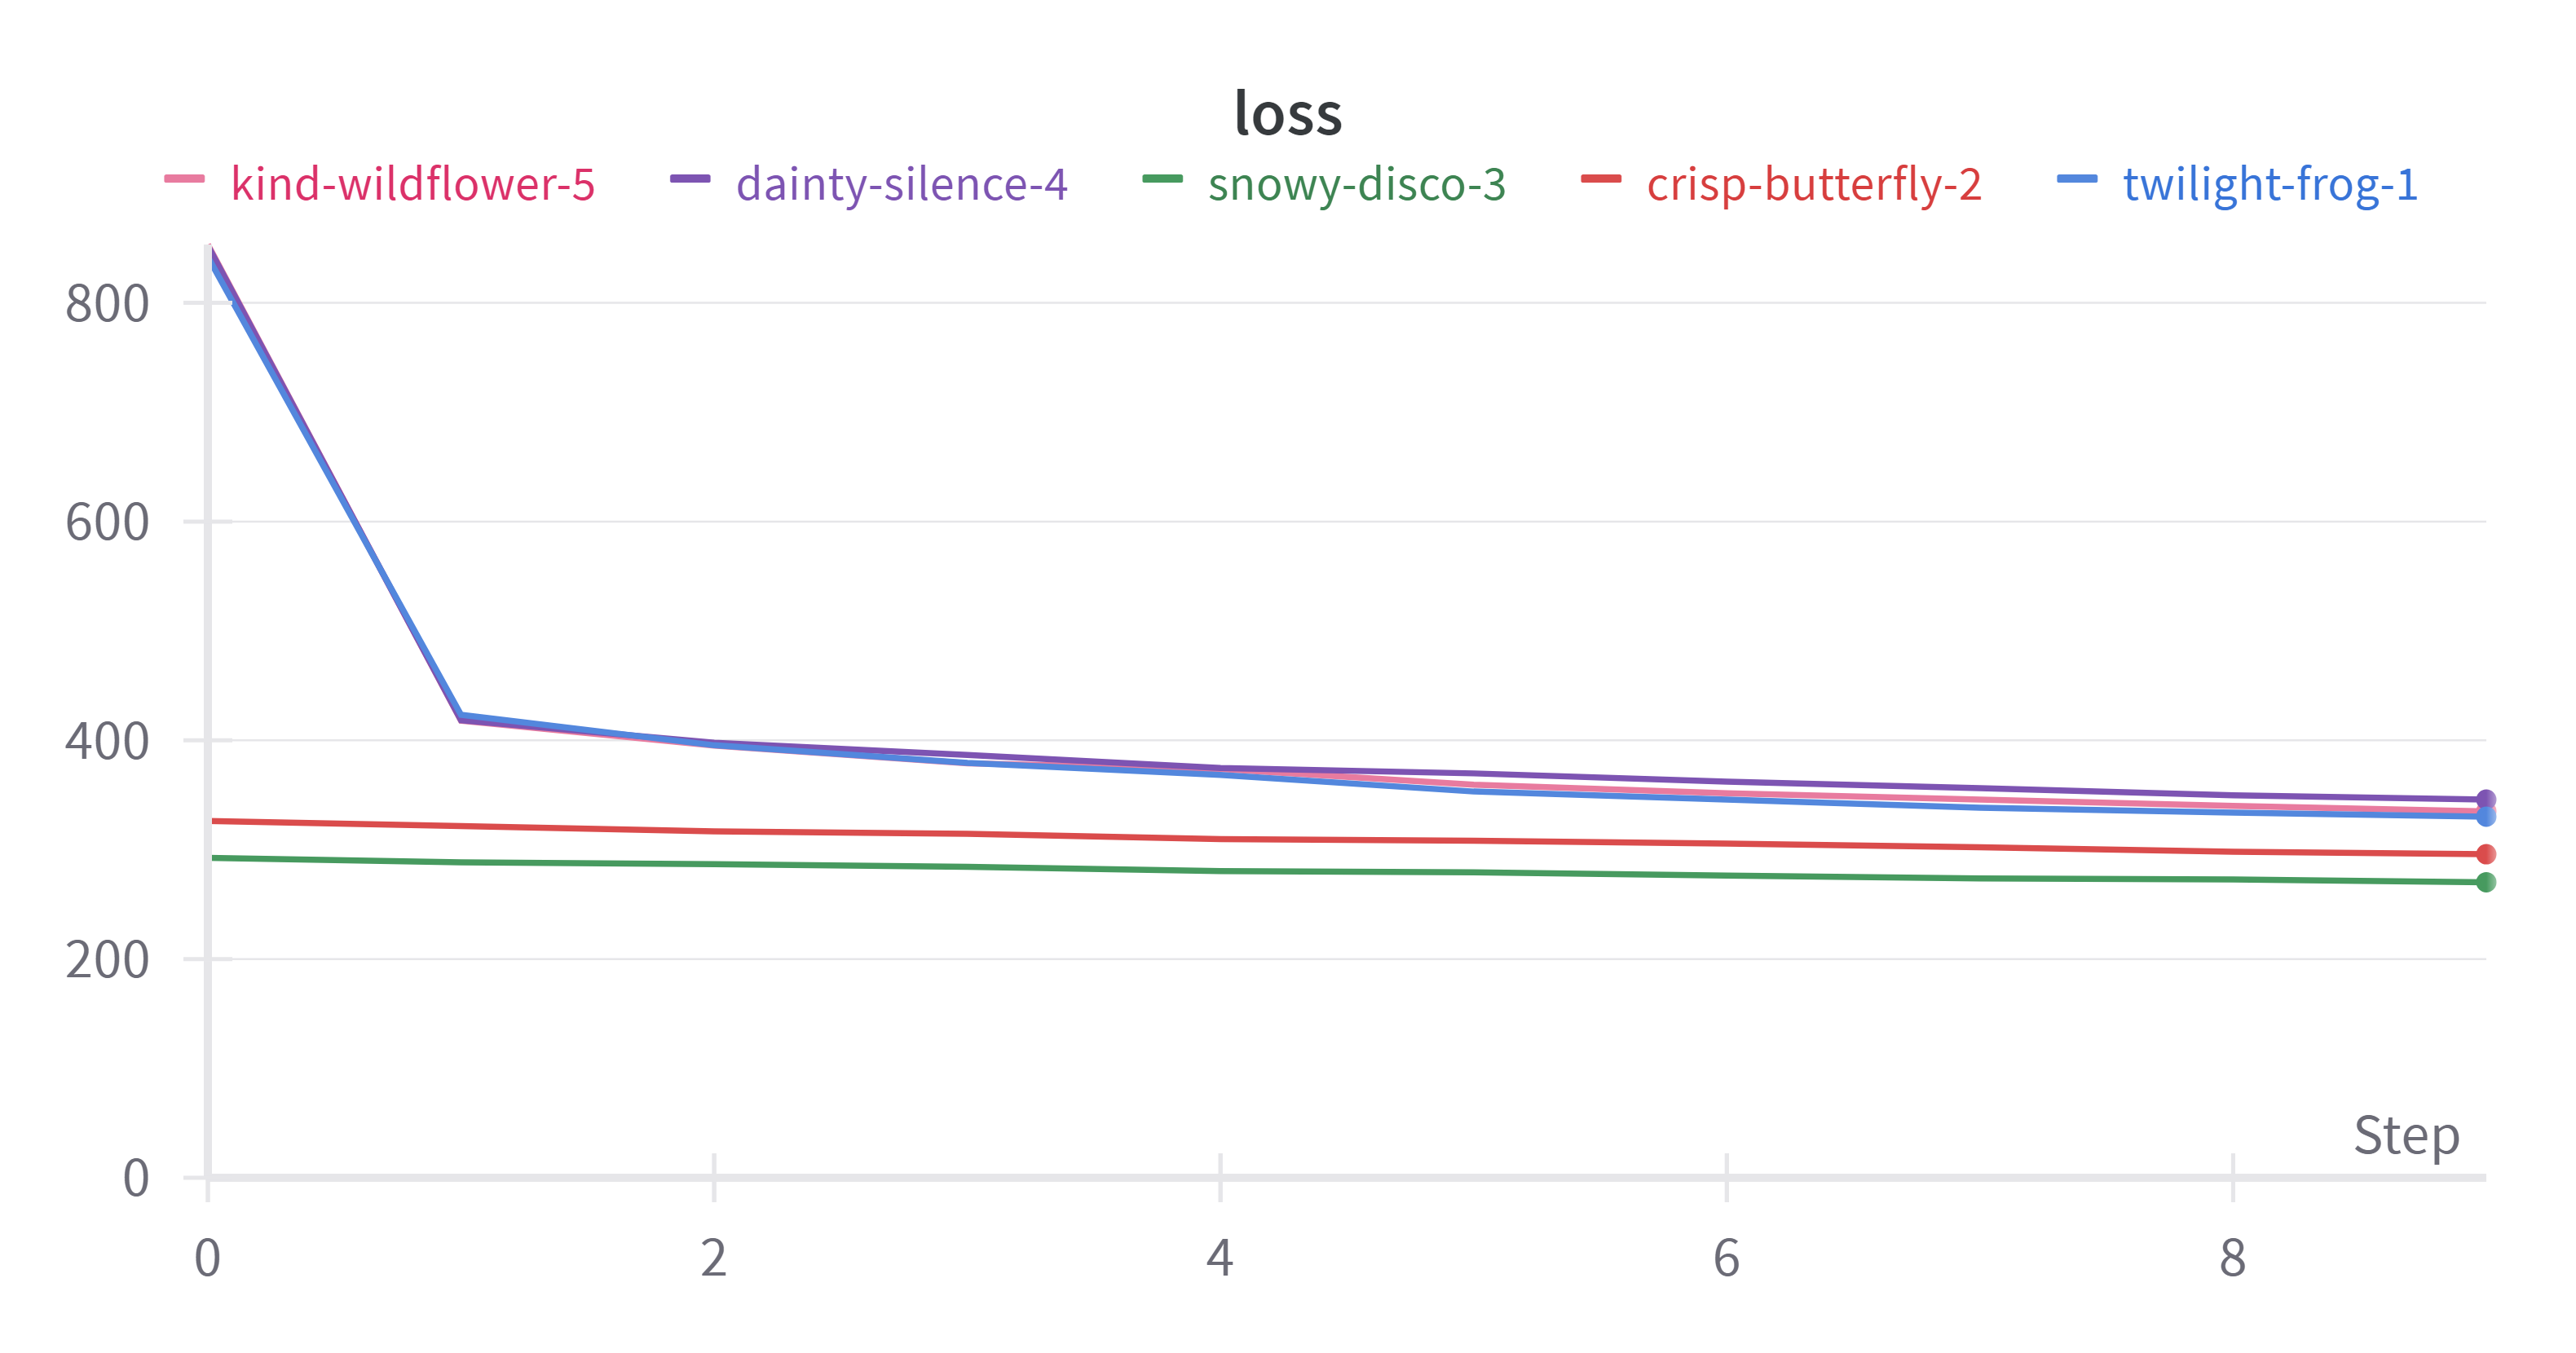
\includegraphics[width=\textwidth]{../figures/wandb_loss_0.png}
    \caption{NN: Training loss by epoch}
\end{figure}

\end{frame}

\begin{frame}
    \begin{figure}
        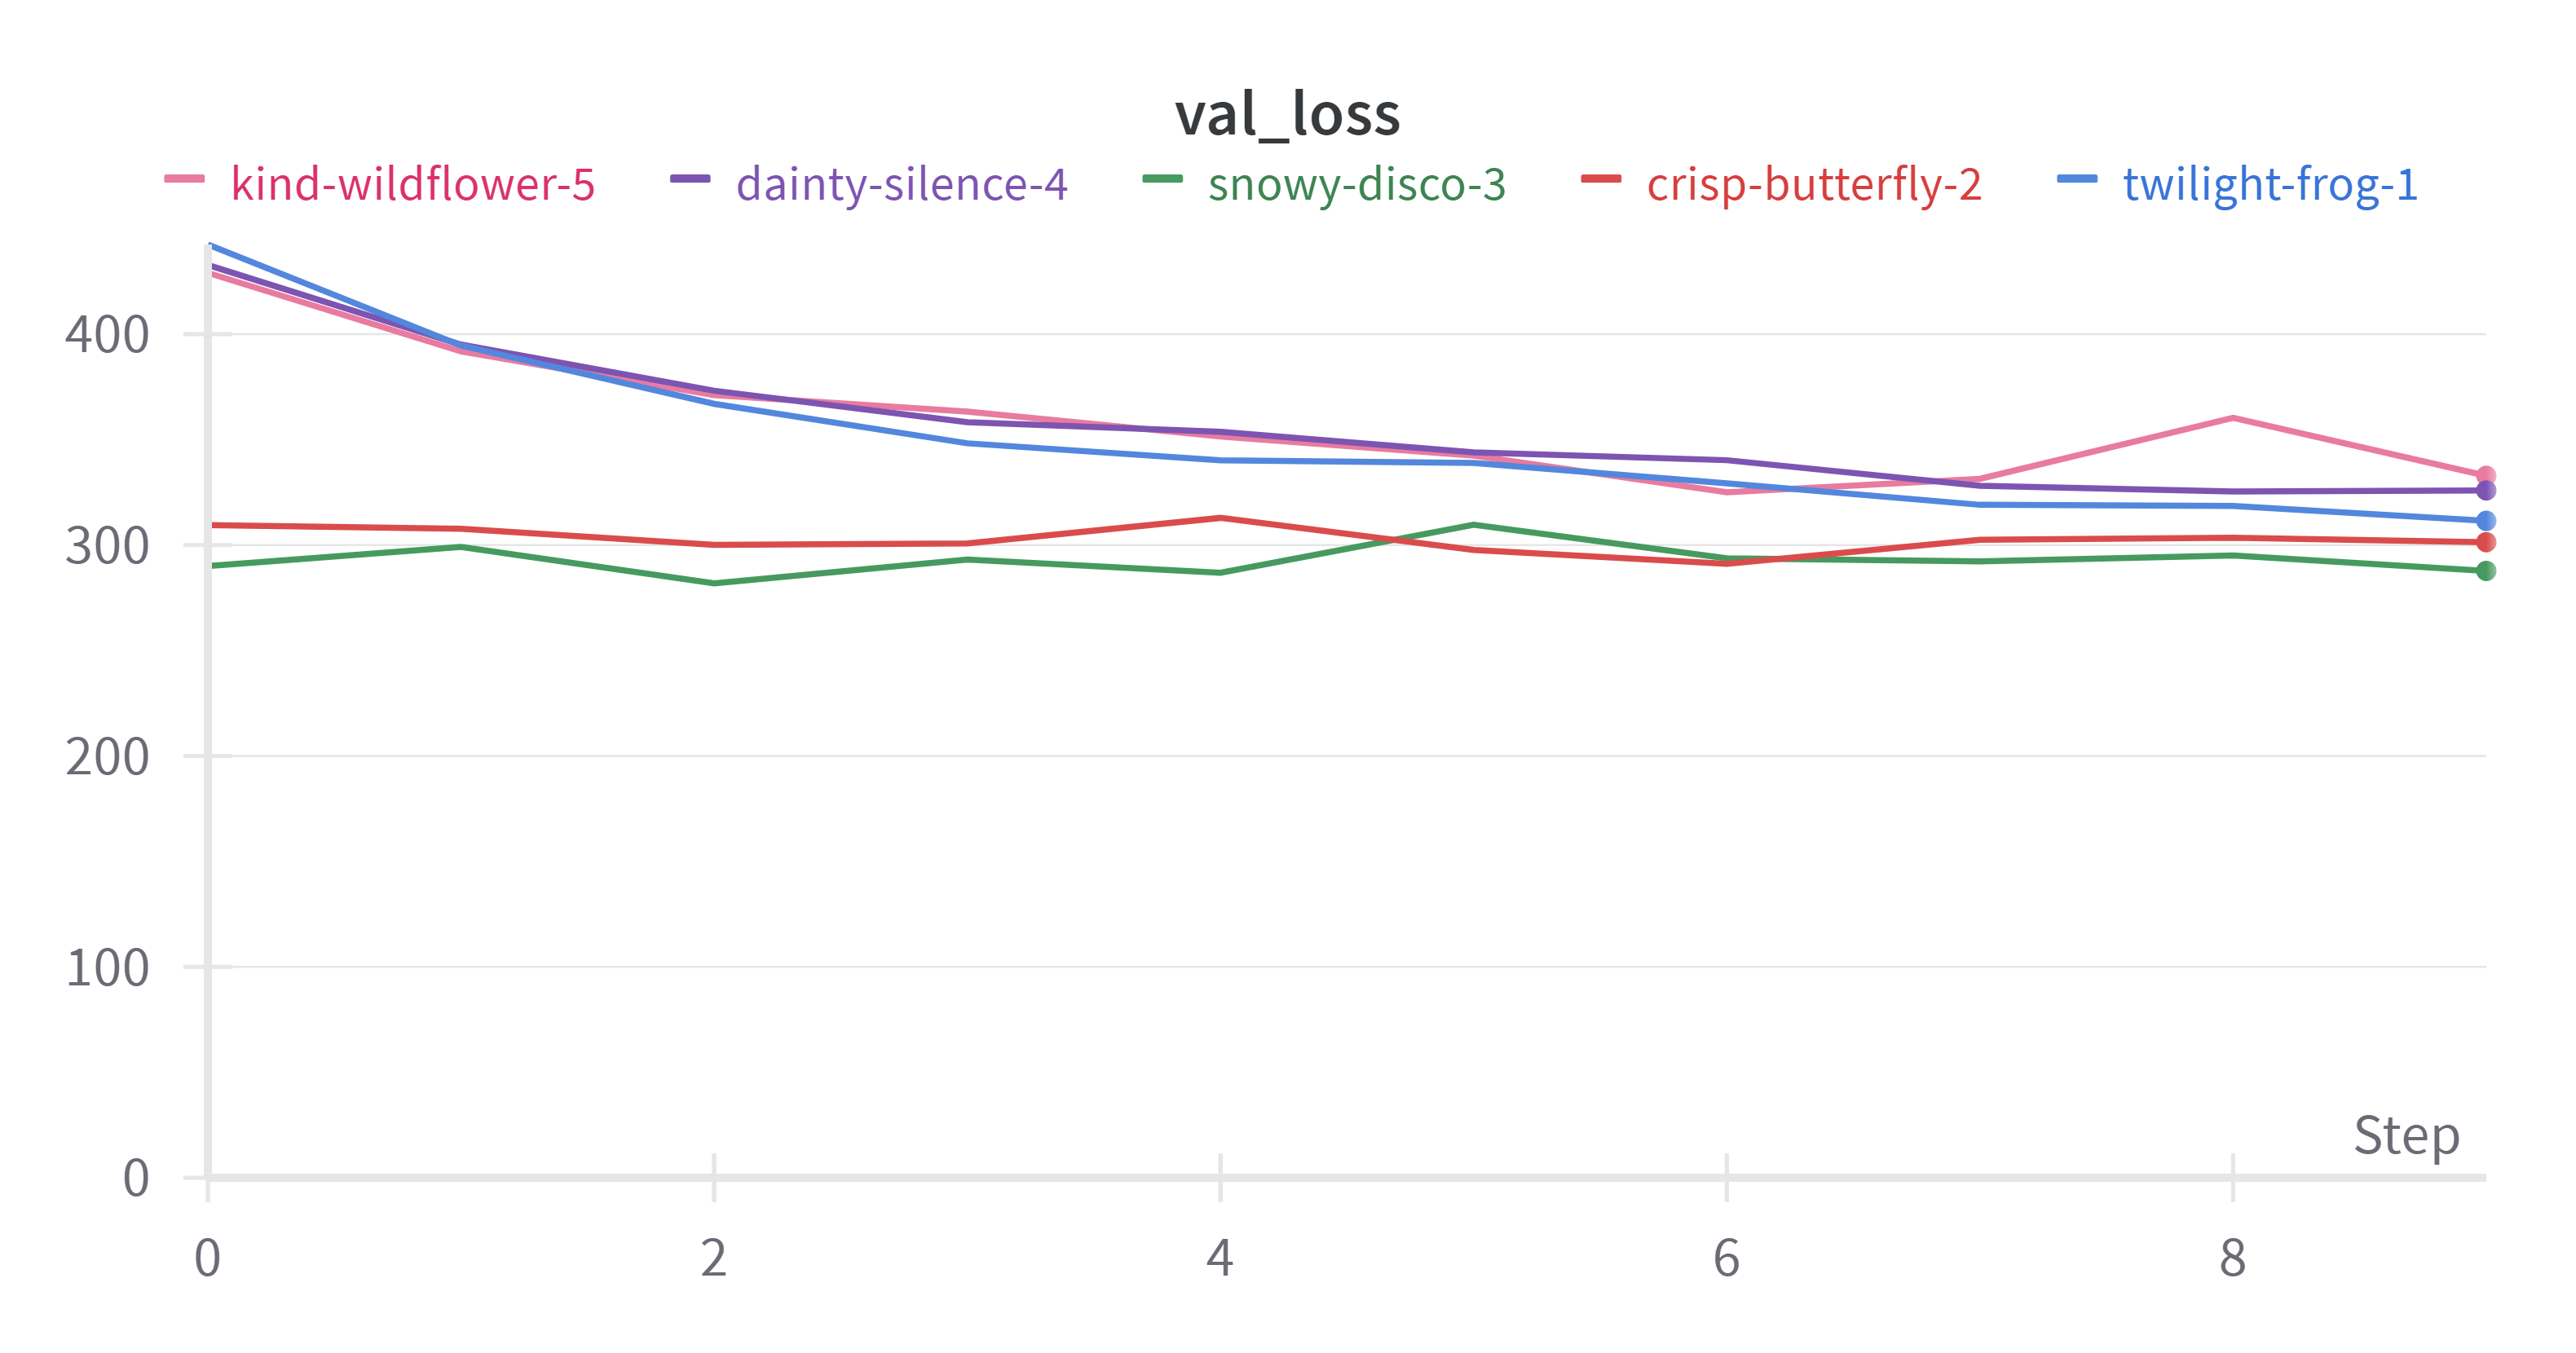
\includegraphics[width=\textwidth]{../figures/wandb_val_loss_0.png}
        \caption{NN: Validation loss by epoch}
    \end{figure}
\end{frame}


\section{Results}

\begin{frame}{Results}
    
    Current performance: tree-based models $>$ neural net $>$ linear models

\begin{table}
    \centering
    \begin{tabular}{|p{8em}|p{8em}|}
        \hline
        \textbf{Model} & \textbf{MSE loss} \\ \hline
        OLS            & 455.8       \\ \hline
        Lasso          & 467.7      \\ \hline
        Ridge          & 455.8       \\ \hline
        Random Forest  & 219.4         \\ \hline
        Gradient Boosting & 209.1       \\ \hline
        FF Neural Net  & 287.8         \\ \hline
    \end{tabular}
\end{table}
\end{frame}


\begin{frame}{Next Steps}
\begin{itemize}
    \item Test modeling pipeline on more collections (Punks, Penguins, Ninjas, etc.)
    \item Implement more neural nets (RNN/LSTM, etc.)
\end{itemize}

\bigskip
Github repo: \url{https://github.com/mingxuan-he/NFT-pred}

\end{frame}



\end{document}